% !TeX spellcheck = en_US
\subsection{Weighted Histogram Analysis Method\label{Sec:FEM:WHAM}}
The weighted histogram analysis method is a generalization of the histogram method developed by Ferrenberg and Swendsen.\cite{FerrenbergPRL1989}
\subsubsection{Weighted Histogram Analysis Method for Parallel Tempering\label{Sec:FEM:WHAM_REMD}}
The following derivation quite follows Ref.~\cite{ChoderaJCTC2007}.
One of the central quantities in statistical mechanics is configurational integral $Z$, which in textbook is often written as
\begin{equation}
Z=\int \exp{(-\beta U(\mathbf{R}))}\diff\mathbf{R}.
\end{equation}
This is an integral in coordinate space. It also can be written as an integral in energy space
\begin{equation}
Z=\int \Omega(U)\exp{(-\beta U)}\diff U,
\end{equation}
where $\Omega(U)$ is density of states and $\Omega(U)\Delta U$ is the number of states in the region $U-\Delta U/2<U<U+\Delta U/2$. Accordingly, the statistical expectation of an operator $\mathbf{A}$ can be calculated by
\begin{equation}
\langle \mathbf{A}\rangle=\frac {\int \mathbf{A}(U)\Omega(U)\exp{(-\beta U)}\diff U}{\int \Omega(U)\exp{(-\beta U)}\diff U},
\end{equation}
where
\begin{equation}
\mathbf{A}(U^\prime)=\frac{\int \delta (U(\mathbf{R})-U^\prime)\mathbf{A}(\mathbf{R})\diff \mathbf{R}}{\int \delta (U(\mathbf{R})-U^\prime)\diff\mathbf{R}},
\end{equation}
is the average of $\mathbf{A}$ over all the samples with an energy $U^\prime$. Therefore, the core objective is to calculate $\Omega(U)$.

Suppose we have one trajectory with $N$ snapshots denoted as $\{\mathbf{R}_n\}$. We then discretize the energy space into $M$ bins with width $\Delta U$, and count the number of snapshots fallen into each bin. For convenience, we define $\psi_m(U)$ as
\begin{equation}
	\psi_m(U)= 
	\left\{ 
	\begin{array}{rl} 
	1 & \text{if }U\in \left[ U_m-\Delta U/2, U_m+\Delta U/2\right)\\ 
	0 & \text{otherwise}\\  
	\end{array} 
	\right. 
\end{equation}
Then the histogram for the $m$th energy bin is
\begin{equation}
	H_{m}=\sum\limits_{n=1}^{N}\psi_{m}(U(\mathbf{R}_n))=N\cdot \frac 1 N\sum\limits_{n=1}^{N}\psi_{m}(U(\mathbf{R}_n))=N\cdot\left<\psi_m\right>,
\end{equation}
with variances (see Appendix~\ref{chapter:Appendix:Uncertainty})
\begin{align}
	\delta^2 H_m=&N^2\delta^2(\left<\psi_m\right>)\notag\\
	            =&g_m N\left(\left<{\psi_m}^2\right>-\left<\psi_m\right>^2\right)\notag\\
	            =&g_m N\left(\left<\psi_m\right>-\left<\psi_m\right>^2\right)\notag\\
	            =&g_m H_m\left(1-\frac{H_m}{N}\right).
\end{align}

A sample histogram in 2D space is shown in Fig.~\ref{Fig:FEM:WHAM:histogram}.
\begin{figure}[htbp]
	\centering
    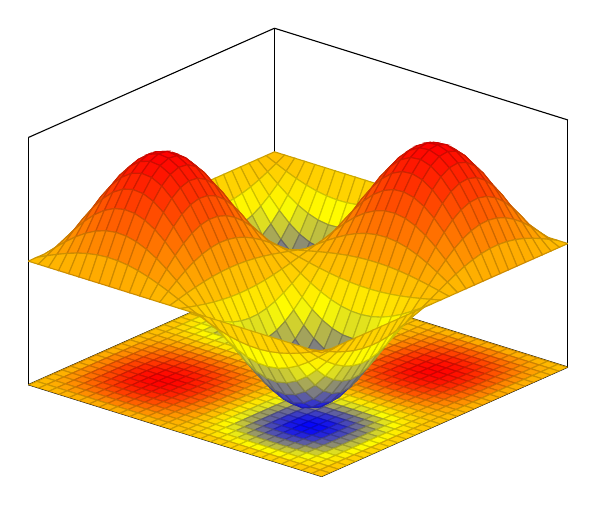
\begin{tikzpicture}
        \begin{axis}[xtick=\empty, ytick=\empty, ztick=\empty, minor tick num=0,view/h=40]
        
          \addplot3[surf,
          mesh/color input=colormap,
          colormap/hot,
          domain=-180:180, y domain=-180:180,
          point meta={sin(x)*sin(y)},
          point meta rel=per plot,
          point meta min=-1.0, point meta max=1.0,
          shader=faceted,
          update limits=false,
          on layer=axis background,
          samples=30
          ] {-1.2};
          \addplot3[surf, shader=faceted, domain=-180:180, y domain=-180:180, samples=30] 
          {sin(x)*sin(y)};
%         \addplot3[surf, shader=faceted, domain=-180:180, y domain=-180:180, samples=20, color=black, point meta rel=per plot, point meta={sin(x)*sin(y)} ] {-1.0};

        \end{axis}
    \end{tikzpicture}
    \caption{A sample histogram in 2D space, for instance potential energy and a reaction coordinate $\xi$.}\label{Fig:FEM:WHAM:histogram}
\end{figure}
%\begin{figure}[htbp]
%	\centering
%	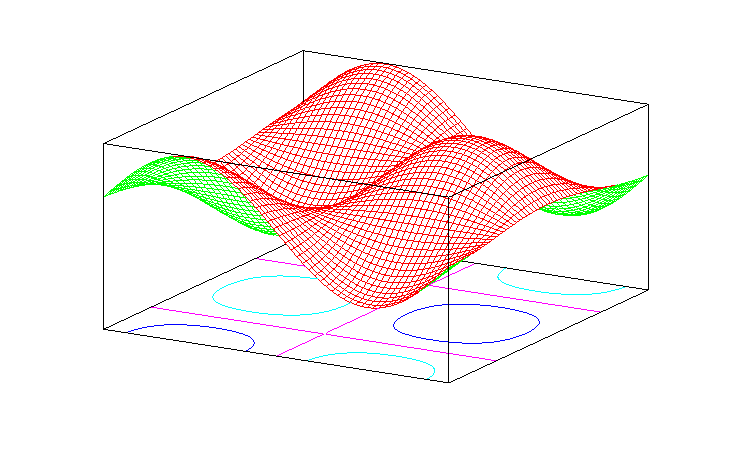
\includegraphics[width=0.8\textwidth]{figures/histogram.pdf}\\
%	\caption{A sample histogram in 2D space, for instance potential energy and a reaction coordinate $\xi$.}\label{Fig:FEM:WHAM:histogram}
%\end{figure}

The ratio of the histogram $H_m$ to the total number of snapshots $N$ divided by the bin width $\Delta U$ can be approximately taken as the probability of states in this bin, i.e.,
\begin{equation}
	\frac{\Omega_m\exp{(-\beta U_m)}}{Z}\approx\frac{H_m}{N\Delta U}.
\end{equation}
Therefore,
\begin{align}
	\Omega_m=&\frac{1}{\Delta U}\cdot\frac{H_m}{N}\cdot\frac{Z(\beta)}{\exp{(-\beta U_m)}}\notag\\
	        =&\frac{H_m}{N\Delta U\exp{\left[f-\beta U_m\right]}},
	\label{Eq:FEM:WHAM:DoSsingle}
\end{align}
and variances
\begin{equation}
	\delta^2\Omega_m=\frac{\delta^2 H_m}{\left(N\Delta U\exp{\left[f-\beta U_m\right]}\right)^2},
\end{equation}
in which we have defined a dimensionless free energy $f=-\ln{Z(\beta)}$.

Practically, we may run multiple ($K$) trajectories using, for example, replica exchange molecular dynamics simulations. For each trajectory (index $k$), we have unique estimators for the histogram $H_{mk}$, the density of states $\Omega_{mk}$ and their variances $\delta^2 H_{mk}$ and $\delta^2\Omega_{mk}$ being
\begin{equation}
	H_{mk}=\sum\limits_{n=1}^{N_k}\psi_{m}(U(\mathbf{R}_{kn})),
\end{equation}
\begin{equation}
	\delta^2 H_{mk}=g_{mk}H_{mk}\left(1-\frac{H_{mk}}{N_k}\right),
\end{equation}
\begin{align}
	\Omega_{mk}=\frac{H_{mk}}{N_k\Delta U\exp{\left[f_k-\beta_kU_{m}\right]}},
	\label{Eq:FEM:WHAM:Omega_mk}
\end{align}
and
\begin{equation}
	\delta^2\Omega_{mk}=\frac{\delta^2 H_{mk}}{\left(N_k\Delta U\exp{\left[f_k-\beta_kU_{m}\right]}\right)^2},
\end{equation}
The optimum estimator of the density of states from all the simulations is
\begin{equation}
	\Omega_m=\frac{\sum\limits_{k=1}^K\left[\delta^2\Omega_{mk}\right]^{-1}\Omega_{mk}}{\sum\limits_{k=1}^K\left[\delta^2\Omega_{mk}\right]^{-1}},
	\label{Eq:FEM:WHAM:optimumOmega}
\end{equation}
which is the weighted average of density of states of all the trajectories with the weight reversely proportional to the uncertainties (see Appendix~\ref{chapter:Appendix:Mean}).

To make the expression simpler, here we take some approximations. First, normally the energy space is split into a large number of bins. The histogram in each bin is much smaller than the total number of snapshots, i.e. $H_{mk}\ll N_k$. The expectation of $H_{mk}$ can be related to the optimum estimator of the density of states, i.e.
\begin{equation}
	\overline{H_{mk}}=N_k\Delta U\Omega_m\exp{(f_k-\beta_kU_m)}.
\end{equation}
Then we have
\begin{equation}
    \delta^2H_{mk}=g_{mk}N_k\Delta U\Omega_m\exp{(f_k-\beta_kU_m)}
    \label{EQ:FEM:WHAM:delta2H_mk}
\end{equation}
and
\begin{equation}
\delta^2\Omega_{mk}=\frac{\Omega_m}{{g_{mk}}^{-1}N_k\Delta U\exp{(f_k-\beta_kU_m)}}.
\label{Eq:FEM:WHAM:delta2Omega_mk}
\end{equation}

Taking Eq.~\ref{Eq:FEM:WHAM:Omega_mk} and Eq.~\ref{Eq:FEM:WHAM:delta2Omega_mk} into Eq.~\ref{Eq:FEM:WHAM:optimumOmega}, we find
\begin{equation}
\Omega_m=\frac{\sum\limits_{k=1}^{K}{g_{mk}}^{-1}H_{mk}}{\sum\limits_{k=1}^{K}{g_{mk}}^{-1}N_k\Delta U\exp{(f_k-\beta_kU_m)}},
\label{Eq:FEM:WHAM:Omega_iteration}
\end{equation}
in which
\begin{equation}
f_k=-\ln\sum\limits_{m=1}^M\Omega_m\Delta U\exp{(-\beta_kU_m)}.
\label{Eq:FEM:WHAM:f_k_iteration}
\end{equation}
Obviously, Eq.~\ref{Eq:FEM:WHAM:Omega_iteration} and Eq.~\ref{Eq:FEM:WHAM:f_k_iteration} must be solved iteratively.
Applying the error propagation rule to Eq.~\ref{Eq:FEM:WHAM:Omega_iteration} and using Eq.~\ref{EQ:FEM:WHAM:delta2H_mk}, the uncertainty of $\Omega_m$ is given by
\begin{equation}
\delta^2 \Omega_m=\frac{\Omega_m}{\sum\limits_{k=1}^K{g_{mk}}^{-1}N_k\Delta U\exp{(f_k-\beta_kU_m)}},
\end{equation}
and the relative uncertainty is given by
\begin{equation}
\frac{\delta^2\Omega_m}{\Omega_m^2}=\left[\sum\limits_{k=1}^K{g_{mk}}^{-1}H_{mk}\right]^{-1}.
\end{equation}
Using the density of states and its variance, we can estimate the expectation of any configuration function $A(\mathbf{R})$ at any inverse temperature $\beta$
\begin{equation}
\left<A\right>_\beta\approx\frac{\sum\limits_{m=1}^M\Omega_m\Delta U\exp{(-\beta U_m)}A_m}{\sum\limits_{m=1}^M\Omega_m\Delta U\exp{(-\beta U_m)}},
\label{Eq:FEM:WHAM:A}
\end{equation}
where
\begin{equation}
A_m=\frac{\int \diff\mathbf{R}A(\mathbf{R})\psi_m(U(\mathbf{R}))}{\int \diff\mathbf{R}\psi_m(U(\mathbf{R}))}.
\end{equation}
Using histograms of bin $m$ from all the simulations and defining $H_m=\sum\limits_{k=1}^KH_{mk}$, an estimator of $A_m$ denoted as $\hat{A}_m$ can be calculated as
\begin{equation}
   \hat{A}_m={H_{m}}^{-1}\sum\limits_{k=1}^K\sum\limits_{n=1}^{N_k}\psi_m(U(\mathbf{R}_{kn}))A(\mathbf{R}_{kn}).
   \label{Eq:FEM:WHAM:A_m}
\end{equation}
Taking Eq.~\ref{Eq:FEM:WHAM:A_m} into Eq.~\ref{Eq:FEM:WHAM:A}, we obtain an estimator of $\hat{A}(\beta)$
\begin{align}
\hat{A}(\beta)=&\frac{\sum\limits_{m=1}^M\Omega_m\Delta U\exp{(-\beta U_m)}{H_{m}}^{-1}\sum\limits_{k=1}^K\sum\limits_{n=1}^{N_k}\psi_m(U(\mathbf{R}_{kn}))A(\mathbf{R}_{kn})}{\sum\limits_{m=1}^M\Omega_m\Delta U\exp{(-\beta U_m)}}\\
              =&\frac{\sum\limits_{m=1}^M\Omega_m\Delta U\exp{(-\beta U_m)}{H_{m}}^{-1}\sum\limits_{k=1}^K\sum\limits_{n=1}^{N_k}\psi_m(U(\mathbf{R}_{kn}))A(\mathbf{R}_{kn})}{\sum\limits_{m=1}^M\Omega_m\Delta U\exp{(-\beta U_m)}{H_{m}}^{-1}\sum\limits_{k=1}^K\sum\limits_{n=1}^{N_k}\psi_m(U(\mathbf{R}_{kn}))}\\
              =&\frac{\sum\limits_{k=1}^K\sum\limits_{n=1}^{N_k}w_{kn}(\beta)A_{kn}}{\sum\limits_{k=1}^K\sum\limits_{n=1}^{N_k}w_{kn}(\beta)},
\end{align}
where the per-configuration weights $w_{kn}(\beta)$ is given by
\begin{equation}
w_{kn}(\beta)=\sum\limits_{m=1}^M{H_{m}}^{-1}\psi_m(U(\mathbf{R}_{kn}))\Omega_m\exp{(-\beta U_m)}
\end{equation}

\subsubsection{Weighted Histogram Analysis Method From Minimizing Statistical Error}
In this section, the ``traditional'' derivation method of WHAM are briefly reviewed.\cite{SouailleCPC2001} In the WHAM, the goal is to get an optimal unbiased probability distribution $\rho_{0}(\eta)$, where $\eta$ is a series of discretized histogram bins indexed by $j=1,2,3,...,M$ along a certain reaction coordinate. WHAM can be used to analyze the Umbrella Sampling (US) simulations, where a set of simulations indexed by $i$ or $k=1,2,3,...,S$ are performed with a series of biasing potentials added on the reaction coordinate $\eta$. To consider a reference molecular system with the potential energy $U_{0}(\textbf{x})$, where $\textbf{x}$ is the set of atomic coordinates. The reaction coordinate $\eta$ is a function of the atomic coordinates, i.e. $\eta(\textbf{x})$. To suppose that the $i$th molecular simulation has been performed using potential energy function
\begin{equation}
U_{i}^{(b)}(\eta) = U_{0}(\textbf{x}) + W_{i}(\eta(\textbf{x})),
\label{Eq:biasmd}
\end{equation}
where $W_{i}(\eta(\textbf{x}))$ is the biasing potential added on the reaction coordinate $\eta$, e.g. $W_{i}(\eta)=\frac{1}{2}k_{i}(\eta-\eta_{i})^2$ in a Harmonic form. From these simulations a set of normalized biased probability distributions ${\rho_{i}^{(b)}(\eta)}$ can be obtained.
\begin{equation}
\rho_{i}^{(b)}(\eta) = \frac{e^{-\beta U_{i}^{(b)}(\eta)}}{Q_{i}^{(b)}},
\label{Eq:bias}
\end{equation}
where $Q_{i}^{(b)}=\int e^{-\beta U_{i}^{(b)}(\eta)} \diff\eta = e^{-\beta f_{i}^{(b)}}$ and $f_{i}^{(b)}$ is the biased free energy.
The corresponding unnormalized unbiased probability distribution $\rho_{i}^{(u)}(\eta)$ from the $i$th simulation is defined as, 
\begin{align}
\rho_{i}^{(u)}(\eta) = e^{\beta[W_{i}(\eta)-f_{i}^{(b)}]}\rho_{i}^{(b)}(\eta)
\label{Eq:unbias}
\end{align}
In the following, the free energy $f_{i}^{(b)}$ is assumed to be known. 
It has been shown that in the WHAM method, the total normalized unbiased probability distribution $\rho_{0}(\eta)$ can be obtained by a linear $\eta$-dependent combination of the unbiased histograms $\rho_{i}^{(u)}(\eta)$ 
\begin{equation}
\rho_{0}(\eta)=C\sum_{i=1}^{S}p_{i}(\eta)\rho_{i}^{(u)}(\eta),
\label{Eq:unbias0}
\end{equation}  
where $C$ is the normalization factor. $p_i$ is the weight to be optimized, which is under a constraint that
\begin{equation}
\sum_{i=1}^{S}p_{i}(\eta)=1.
\label{Eq:p1}
\end{equation}
These weights are chosen so as to minimize the statistical error made on the total unbiased probability distribution $\rho_{0}(\eta)$, that is, for any given value of $\eta$,
\begin{equation}
\frac{\partial(\sigma^2[\rho_{0}(\eta)])}{\partial p_{i}(\eta)}=0.
\label{Eq:partialp}
\end{equation} 
It can be easily found that $\rho_{0}(\eta)$ satisfy
\begin{align}
\rho_{0}(\eta) = & C\sum_{i=1}^{S}\frac{N_{i}e^{-\beta[W_{i}(\eta)-f_{i}^{(b)}]}}{\sum_{k=1}^{S}N_{k}e^{-\beta[W_{k}(\eta)-f_{k}^{(b)}]}}\rho_{i}^{(u)}(\eta) \notag\\
= & C\sum_{i=1}^{S}\frac{N_{i}}{\sum_{k=1}^{S}N_{k}e^{-\beta[W_{k}(\eta)-f_{k}^{(b)}]}}\rho_{i}^{(b)}(\eta) \notag\\
= & C\frac{\sum_{i=1}^{S}N_{i}\rho_{i}^{(b)}(\eta)}{\sum_{k=1}^{S}N_{k}e^{-\beta[W_{k}(\eta)-f_{k}^{(b)}]}},
\label{Eq:unbias02}
\end{align} 
where $\rho_{i}^{(b)}(\eta)$ can be written as a $\delta$ function,
\begin{equation}
\rho_{i}^{(b)}(\eta) \equiv \frac{1}{N_{i}} \sum_{l=1}^{N_{i}} \delta {(\eta-\eta_{i,l})},
\label{Eq:delta01}
\end{equation} 
where $\eta_{i,l}$ is the reaction coordinates of the $l$th configuration in the $i$th biased simulation .

Until now, the treatment assumes that the free energy parameters ${f_{i}^{(b)}}$ are known. In fact, these parameters can be obtained self-consistently. Indeed, the definition of the free energy $f_{i}^{(b)}$ is,
\begin{align}
e^{-\beta f_{i}^{(b)}}=&\int e^{-\beta U_{i}^{(b)}(\eta) } \diff\eta \notag\\
=&\int \rho_{0}(\eta) e^{-\beta W_{i}(\eta)} \diff\eta \notag\\
=&C \int \frac{\sum_{i=1}^{S}N_{i}\rho_{i}^{(b)}(\eta)}{\sum_{k=1}^{S}N_{k}e^{-\beta[W_{k}(\eta)-f_{k}^{(b)}]}}e^{-\beta W_{i}(\eta)}  \diff\eta
\label{Eq:fi01}
\end{align} 
The set of parameters ${f_{i}^{(b)}}$ appear on both sides of Eq.~\ref{Eq:fi01}, which must be solved iteratively. A initial guess of the values ${f_{i}^{(b)0}}$ is used on the right side of Eq.~\ref{Eq:fi01} to compute a new set of values ${f_{i}^{(b)1}}$, which is in turn used as the new guess to compute ${f_{i}^{(b)1}}$ and so on until convergence is reached. Then, the unbiased free energy corresponding to the histogram can be calculated by,
\begin{equation}
f_{0}(\eta)=-\beta^{-1}\ln \rho_{0}(\eta) 
\label{Eq:f0}
\end{equation} 
To get rid of the constant $C$ in the Eq.~\ref{Eq:unbias02}, one may subtract the offset constant $f_{0}(\eta_{1})$ from all the $f_{0}(\eta_{j})$.  

\subsubsection{Weighted Histogram Analysis Method From Maximum Likelihood}
The following derivation quite follows Ref.~\cite{GallicchioJPCB2005}, in which maximum likelihood principle is utilized. 
Suppose we have performed $K$ simulations, each at a different inverse temperature $\beta_k$ and possibly with different biasing potential $w_k(\mathbf{R})$.
We then discretize the 2D plane spanned by the coordinate and unbiased potential energy into bins, each characterized by ${\mathbf{R}_j}$ and ${E_h}$. To make the following derivation cleaner, we map the 2D bins to one dimensional series with index $l, l=1,\dots,L$. Next, we construct histograms for bins using all the samples from the simulations. The probability of finding the system in bin $l$ during the $k$th simulation can be written as
\begin{equation}
p_{k,l}=f_kc_{k,l}p_l^0,
\end{equation}
in which $p_l^0$ is the (simulation-independent) unbiased probability,
\begin{align}
c_{k,l}=&\exp{\left[-\beta_k\left(E_l+w_{k,l}\right)+\beta_0E_l\right]}\notag\\
=&\exp{\left[-\left(\beta_k-\beta_0\right)E_l\right]}\exp{\left(-\beta_kw_{i,l}\right)}
\end{align}
is the bias factor, $E_l$ is the unbiased energy of bin $l$, $f_k={\left\{\sum\limits_lc_{k,l}p_l^0\right\}}^{-1}$ is the normalization factor.
It is worth emphasizing that the biasing potential can be multiple dimensional as, for instance, in a two-dimensional umbrella sampling.
If the biasing is only in temperature-space as in replica exchange molecular dynamics
\begin{equation}
c_{k,l}=\exp{\left[-\left(\beta_k-\beta_0\right)E_l\right]},
\end{equation} 
while if the biasing is only in potential as in umbrella sampling
\begin{equation}
c_{k,l}=\exp{\left(-\beta_0w_{k,l}\right)}.
\end{equation}

If we assume that each count in each histogram is independent, then the likelihood of observing the $k$th histogram distribution is given by the multinomial distribution
\begin{align}
P(n_{k,1},n_{k,2},\dots,n_{k,L}|p_{k,1},p_{k,2},\dots,p_{k,L})=\notag\\
\frac{\left(\sum\limits_l n_{k,l}\right)!}{\prod\limits_l n_{k,l}!}\prod\limits_{l=1}^L\left(p_{k,l}\right)^{n_{k,l}}\propto\prod\limits_{l=1}^{L}\left(f_kc_{k,l}p_l^0\right)^{n_{k,l}}.
\end{align}
For all $K$ simulations, the likelihood is the product of multinomial
\begin{align}
P(n_{1,1},\dots,n_{1,L};\dots;n_{K,1},\dots,n_{K,L}|p_1^0,\dots,p_L^0)\propto\notag\\
\prod\limits_{k=1}^K\prod\limits_{l=1}^{L}\left(f_kc_{k,l}p_l^0\right)^{n_{k,l}},
\label{Eq:FEM:WHAM:totalProb}
\end{align}
where the likelihood is conditional only on the unbiased probabilities $p_l^0$, since the bias factors $c_{k,l}$ are known parameters, and the normalization constants $f_k$ are known conditional on $p_l^0$. The maximum likelihood estimate of the unbiased probabilities can be found by maximizing $P$ in Eq.~\ref{Eq:FEM:WHAM:totalProb} with respect to $p_1^0,\dots,p_L^0$ and are given by solutions of the simultaneous nonlinear equations
\begin{equation}
p_l^0=\frac{\sum\limits_{k=1}^K n_{k,l}}{\sum\limits_{k=1}^K N_kf_kc_{k,l}}\, (\text{for each }l)
\end{equation}
and
\begin{equation}
f_k={\left\{\sum\limits_lc_{k,l}p_l^0\right\}}^{-1},
\end{equation}
where $N_k$ is the total number of counts in the $k$th histogram.
